% Main file

%==========================================================================
%  Document Definition
%--------------------------------------------------------------------------
\documentclass[10pt,a4paper]{article}
%==========================================================================

%==========================================================================
% Include Used Packages
%--------------------------------------------------------------------------
\usepackage[utf8]{inputenc}		        	% Keybord settings
\usepackage{titlesec}						% for vertical alignment of (sub-)section titles and title spacing
\usepackage{setspace}						% for line spacing
\usepackage{amsmath}                 		% Additional math functionality
\usepackage{amssymb}						% Additional math symbols
\usepackage[english]{babel}					% for hyphenation and special caracters
\usepackage{graphicx}						% for including images

\usepackage{pst-pdf}						% for latex to pdf
\usepackage{pst-eucl}						% for latex to ps
\usepackage{pst-text}						% for latex to ps
\usepackage{pstricks}						% for inkScape files; for latex to ps

\usepackage{listings}
\usepackage{xcolor}
% Always the last package:
\usepackage[breaklinks]{hyperref}			% Hyperreferenzen für pdf
%==========================================================================

%==========================================================================
% Font
%--------------------------------------------------------------------------
%\usepackage[T1]{fontenc}					% font encoding
%\usepackage{lmodern}						% font
%\renewcommand*\familydefault{\sfdefault}	% Only if the base font of the document is to be sans serif
%==========================================================================

%==========================================================================
% Include modified and customized Commands
%--------------------------------------------------------------------------
% Paragraph with \newline
\titleformat{\paragraph}[display]{\normalfont\bf\normalsize}{\theparagraph}{-2em}{}[]
% No indent after new paragraph
\setlength{\parindent}{0pt}
% Change vertical spacing between paragraphs
\setlength{\parskip}{5pt}
%==========================================================================

%==========================================================================
% Document Infos
%--------------------------------------------------------------------------
\title {
\includegraphics[height=1.40in]{icon.pdf} \\RoboEarth App Engine }
\author {Dominique Hunziker, Mohanarajah Gajamohan, Markus Waibel}
\date{Zurich, \today}
\hypersetup{
	pdftitle={framework},
	pdfauthor={Dominique Hunziker},
	pdfsubject={Specification of reappengine}}
%==========================================================================

%==========================================================================
% Line Spacing
%--------------------------------------------------------------------------
%\onehalfspacing
%==========================================================================

%==========================================================================
% Title Spacing
%--------------------------------------------------------------------------
\titlespacing{\section}{0pt}{10pt}{5pt}
\titlespacing{\subsection}{0pt}{8pt}{4pt}
\titlespacing{\subsubsection}{0pt}{6pt}{0pt}
\titlespacing{\paragraph}{0pt}{6pt}{-2pt}
%==========================================================================

%==========================================================================
% Document Content
%--------------------------------------------------------------------------


\begin{document}
\maketitle
\section*{Introduction}

		Computational power is a key enabler for 
		intelligent and efficient robot task performance. However, on-board
		computation entails additional power requirements, which may constrains robot mobility and operating duration and increases costs.

The RoboEarth App Engine makes powerful computation available to robots. 
It allows users to run their ROS software in the Cloud in a Software as a Service framework with minimal configuration.
In addition,
		keeping the open source and RoboEarth spirit, robots can share compatible 'cloud-apps'.

The RoboEarth App Engine takes advantage of the rapid increase in mobile data transfer rates provided
		by the upcoming LTS standard (down-link peak rates of 300 Mbit/s,
		up-link peak rates of 75 Mbit/s) and the growing number of
		repositories and packages (3350 pkgs at the time of count) available
		under the ROS framework. 
				
In addition, it sidesteps severe drawbacks of client-side robot apps, including high computational costs, 
configuration/setup overheads, dependence on custom middleware, as well as maintenance and update overheads. 
		
	
	\section*{RoboEarth App Engine Framework}
		The RoboEarth App Engine Framework allows users to select, launch and use apps.
		The Django interface of the framework acts as an interpreter between user
		requests and their apps. It allows 
communication with processes using \textsc{ROS}, process management
		using \emph{roslaunch} and has a standardized language to communicate between
		processes. In this first implementation we focused on the usage of \emph{nodes} which provide
		\emph{services} as apps.
		
		The client interface of the framework communicates with app users. 
To include a broader audience the interaction uses the standard \textsc{http} protocol.
		This allows users who do not have \textsc{ROS} and opens the door to using apps from
		a web browser by using the framework as a web server. For this first
		implementation the focus is on the robots as users. For the API 
		the implementation \emph{django}/\emph{piston} was used.
	
	\section*{Requirements}
		Apps have to be \textsc{ROS} \emph{nodes} providing a
		\emph{service} which can be used by the user. No further restrictions are
		necessary.
		
		For the communication between the user and the framework the \textsc{http} protocol (request types \textsc{GET}, \textsc{POST} and \textsc{DELETE}) is used.
		To further
		distinguish and control the interaction dynamic URL are used. This leads basically to
		three levels, i.e. \emph{Service}, \emph{Environment} and \emph{Task}, which results in the
		following URL pattern
		\begin{lstlisting}
BASE/api/reappengine/[envID/[taskID/[fileRef/]]]
		\end{lstlisting}
		The level \emph{Service} represents the entry point for a new user. The first step is to
		create a new environment which essentially creates a new \emph{namespace} in \textsc{ROS}.
		Also on this level the user can add or remove \emph{nodes} from his environment and access general information.
		
		On the next level the user can create a task which is essentially the input message for
		the selected \textsc{ROS} \emph{service}. Again, he can get some information specific to
		his current environment.
		
		And on the last level the user can retrieve the status or, if the task has been completed
		successfully, the result of a task. The forth level \emph{fileRef} is only used to provide
		the possibility to download referenced files for the tasks result, e.g. an image file. The
		result is basically the response message of the selected service.
		
		To exchange the data needed for all these requests the \textsc{json} format is used. Since
		the requests which create a new environment/node or task are implemented as a
		\textsc{POST}, it is also possible to send files. To simplify the construction of requests and
		the interpretation of the responses a small Python-based ServiceAPI is available. For a graphical
		representation of these interactions refer to figure \ref{fig:diagram}. 
		
		\begin{figure}
			\begin{center}
				\def\svgwidth{\columnwidth}
				%%% Creator: Inkscape inkscape 0.48pre0, www.inkscape.org
%% PDF/EPS/PS + LaTeX output extension by Johan Engelen, 2010
%% Accompanies image file 'frameworkOverview' (pdf, eps, ps)
%%
%% To include the image in your LaTeX document, write
%%   \input{<filename>.tex}
%%  instead of
%%   \includegraphics{<filename>.pdf}
%% To scale the image, write
%%   \def{\svgwidth}{<desired width>}
%%   \input{<filename>.tex}
%%  instead of
%%   \includegraphics[width=<desired width>]{<filename>.pdf}

\begingroup
  \makeatletter
  \providecommand\color[2][]{%
    \errmessage{(Inkscape) Color is used for the text in Inkscape, but the package 'color.sty' is not loaded}
    \renewcommand\color[2][]{}%
  }
  \providecommand\transparent[1]{%
    \errmessage{(Inkscape) Transparency is used (non-zero) for the text in Inkscape, but the package 'transparent.sty' is not loaded}
    \renewcommand\transparent[1]{}%
  }
  \providecommand\rotatebox[2]{#2}
  \ifx\svgwidth\undefined
    \setlength{\unitlength}{348.6875pt}
  \else
    \setlength{\unitlength}{\svgwidth}
  \fi
  \global\let\svgwidth\undefined
  \makeatother
  \begin{picture}(1,1.00224054)%
    \put(0,0){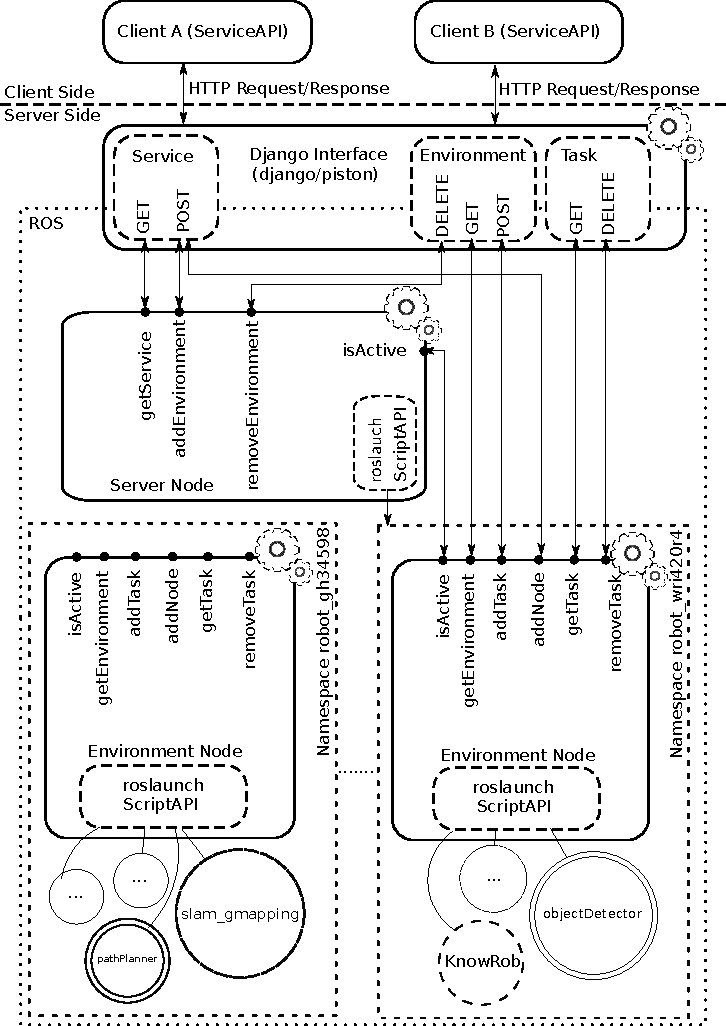
\includegraphics[width=\unitlength]{frameworkOverview}}%
    \put(0.16421171,0.95050233){\makebox(0,0)[lb]{\smash{Client}}}%
    \put(0.23751574,0.95050233){\makebox(0,0)[lb]{\smash{A}}}%
    \put(0.26711216,0.95050233){\makebox(0,0)[lb]{\smash{(ServiceAPI)}}}%
    \put(0.30006286,0.8803048){\makebox(0,0)[lb]{\smash{HTTPRequest}}}%
    \put(0.59347745,0.95050233){\makebox(0,0)[lb]{\smash{Client}}}%
    \put(0.66678149,0.95050233){\makebox(0,0)[lb]{\smash{B}}}%
    \put(0.69534621,0.95050233){\makebox(0,0)[lb]{\smash{(ServiceAPI)}}}%
    \put(0.72864146,0.8803048){\makebox(0,0)[lb]{\smash{HTTPRequest
Client-side}}}%
    \put(0.01425655,0.82075004){\makebox(0,0)[lb]{\smash{Server-side}}}%
    \put(0.35830986,0.78110709){\makebox(0,0)[lb]{\smash{WebAPI
(django/piston)}}}%
    \put(0.03850488,0.68743296){\makebox(0,0)[lb]{\smash{ROS}}}%
    \put(0.18966315,0.78396639){\makebox(0,0)[lb]{\smash{Service}}}%
    \put(0.20686279,0.68679629){\rotatebox{90}{\makebox(0,0)[lb]{\smash{get
post}}}}%
    \put(0.53012273,0.78396639){\makebox(0,0)[lb]{\smash{Environment}}}%
    \put(0.56400981,0.68687659){\rotatebox{90}{\makebox(0,0)[lb]{\smash{delete
get
post}}}}%
    \put(0.74560508,0.78396639){\makebox(0,0)[lb]{\smash{Task}}}%
    \put(0.74972911,0.68679629){\rotatebox{90}{\makebox(0,0)[lb]{\smash{get
delete}}}}%
    \put(0.20651893,0.44619976){\rotatebox{90}{\makebox(0,0)[lb]{\smash{getService}}}}%
    \put(0.25750011,0.37852312){\rotatebox{90}{\makebox(0,0)[lb]{\smash{addEnvironment}}}}%
    \put(0.3517854,0.33945375){\rotatebox{90}{\makebox(0,0)[lb]{\smash{removeEnvironment}}}}%
    \put(0.18932703,0.30110136){\makebox(0,0)[lb]{\smash{ServerNode}}}%
    \put(0.19139192,0.2496725){\makebox(0,0)[lb]{\smash{ROSLaunch
(scriptapi)}}}%
    \put(0.60652352,0.38402661){\rotatebox{90}{\makebox(0,0)[lb]{\smash{getEnvironment}}}}%
    \put(0.64893399,0.46669376){\rotatebox{90}{\makebox(0,0)[lb]{\smash{addTask}}}}%
    \put(0.70036399,0.46037865){\rotatebox{90}{\makebox(0,0)[lb]{\smash{addNode}}}}%
    \put(0.74938497,0.47219725){\rotatebox{90}{\makebox(0,0)[lb]{\smash{getTask}}}}%
    \put(0.80608043,0.42762439){\rotatebox{90}{\makebox(0,0)[lb]{\smash{removeTask}}}}%
    \put(0.55724444,0.34931645){\makebox(0,0)[lb]{\smash{isActive
EnvironmentNode}}}%
    \put(0.81166623,0.30110222){\makebox(0,0)[lb]{\smash{A}}}%
    \put(0.64854109,0.2496725){\makebox(0,0)[lb]{\smash{ROSLaunch
(scriptapi)}}}%
    \put(0.18398902,0.06475908){\makebox(0,0)[lb]{\smash{Node}}}%
    \put(0.25075396,0.06475908){\makebox(0,0)[lb]{\smash{A/a}}}%
    \put(0.47005175,0.06475908){\makebox(0,0)[lb]{\smash{Node}}}%
    \put(0.53681669,0.06475908){\makebox(0,0)[lb]{\smash{A/b}}}%
    \put(0.7557689,0.06475908){\makebox(0,0)[lb]{\smash{Node}}}%
    \put(0.82253384,0.06475908){\makebox(0,0)[lb]{\smash{A/c}}}%
    \put(0.92785709,0.45130175){\rotatebox{90}{\makebox(0,0)[lb]{\smash{Namespace}}}}%
    \put(0.92785709,0.58448634){\rotatebox{90}{\makebox(0,0)[lb]{\smash{A}}}}%
  \end{picture}%
\endgroup

				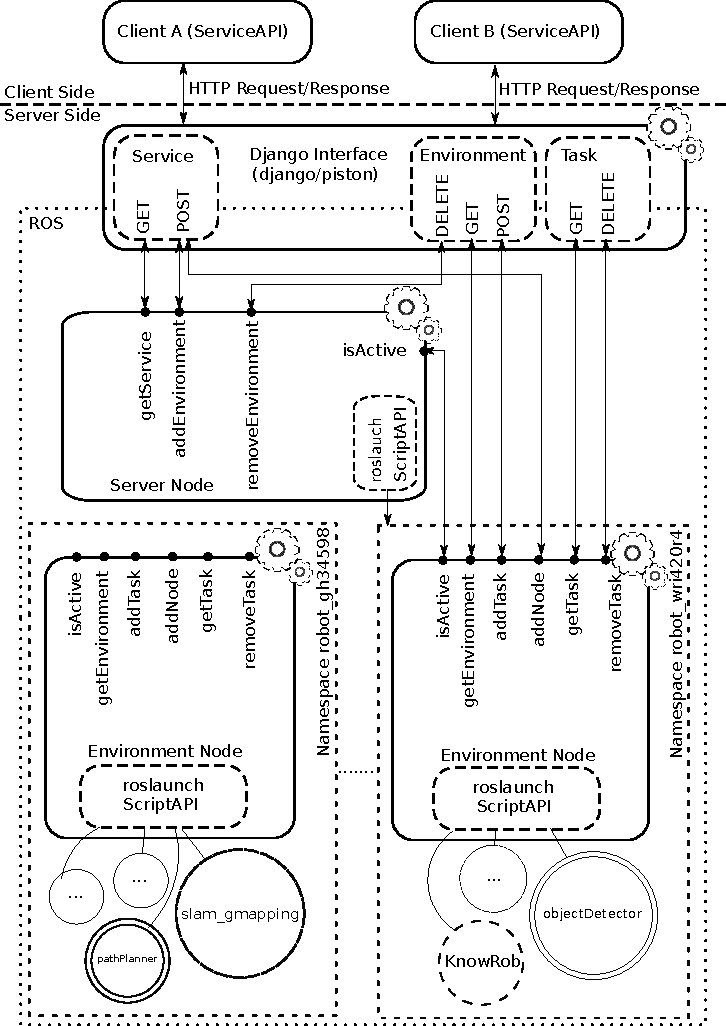
\includegraphics{frameworkOverview.pdf}				
				\caption{Organization of the framework (loosely from top to bottom): The client,
				which can use the provided \emph{ServiceAPI}, communicates with the
				\emph{Django Interface} over \textsc{http}. The \emph{Django Interface} then uses the
				necessary \emph{services} of the \emph{Server Node} or \emph{Environment Node} (solid
				arrows). The \emph{Environment Node} is created and managed by the \emph{Server Node}
				(dashed arrow). The user selected app-\emph{nodes} are then launched and managed by
				the \emph{Environment Node} (dashed arrow) which also provides the necessary
				\emph{services} to create tasks and retrieve their results (solid arrow).}
				\label{fig:diagram}
			\end{center}
		\end{figure}

\end{document}
%==========================================================================
